\documentclass[10pt,a4paper,onecolumn]{article}
\usepackage{marginnote}
\usepackage{graphicx}
\usepackage{xcolor}
\usepackage{authblk,etoolbox}
\usepackage{titlesec}
\usepackage{calc}
\usepackage{tikz}
\usepackage{hyperref}
\hypersetup{colorlinks,breaklinks,
            urlcolor=[rgb]{0.0, 0.5, 1.0},
            linkcolor=[rgb]{0.0, 0.5, 1.0}}
\usepackage{caption}
\usepackage{tcolorbox}
\usepackage{amssymb,amsmath}
\usepackage{ifxetex,ifluatex}
\usepackage{seqsplit}
\usepackage{fixltx2e} % provides \textsubscript
\usepackage[
  backend=biber,
%  style=alphabetic,
%  citestyle=numeric
]{biblatex}
\bibliography{ms\_refs.bib}



% --- Page layout -------------------------------------------------------------
\usepackage[top=3.5cm, bottom=3cm, right=1.5cm, left=1.0cm,
            headheight=2.2cm, reversemp, includemp, marginparwidth=4.5cm]{geometry}

% --- Default font ------------------------------------------------------------
% \renewcommand\familydefault{\sfdefault}

% --- Style -------------------------------------------------------------------
\renewcommand{\bibfont}{\small \sffamily}
\renewcommand{\captionfont}{\small\sffamily}
\renewcommand{\captionlabelfont}{\bfseries}

% --- Section/SubSection/SubSubSection ----------------------------------------
\titleformat{\section}
  {\normalfont\sffamily\Large\bfseries}
  {}{0pt}{}
\titleformat{\subsection}
  {\normalfont\sffamily\large\bfseries}
  {}{0pt}{}
\titleformat{\subsubsection}
  {\normalfont\sffamily\bfseries}
  {}{0pt}{}
\titleformat*{\paragraph}
  {\sffamily\normalsize}


% --- Header / Footer ---------------------------------------------------------
\usepackage{fancyhdr}
\pagestyle{fancy}
\fancyhf{}
%\renewcommand{\headrulewidth}{0.50pt}
\renewcommand{\headrulewidth}{0pt}
\fancyhead[L]{\hspace{-0.75cm}\includegraphics[width=5.5cm]{C:/Users/BryanMaitland/AppData/Local/R/win-library/4.4/rticles/rmarkdown/templates/joss/resources/JOSS-logo.png}}
\fancyhead[C]{}
\fancyhead[R]{}
\renewcommand{\footrulewidth}{0.25pt}

\fancyfoot[L]{\footnotesize{\sffamily Sparks et al., (2025). hatchR: A
toolset to predict hatch and emergence phenology in wild
fishes. \textit{Journal of Open Source Software}, (), . \href{https://doi.org/}{https://doi.org/}}}


\fancyfoot[R]{\sffamily \thepage}
\makeatletter
\let\ps@plain\ps@fancy
\fancyheadoffset[L]{4.5cm}
\fancyfootoffset[L]{4.5cm}

% --- Macros ---------

\definecolor{linky}{rgb}{0.0, 0.5, 1.0}

\newtcolorbox{repobox}
   {colback=red, colframe=red!75!black,
     boxrule=0.5pt, arc=2pt, left=6pt, right=6pt, top=3pt, bottom=3pt}

\newcommand{\ExternalLink}{%
   \tikz[x=1.2ex, y=1.2ex, baseline=-0.05ex]{%
       \begin{scope}[x=1ex, y=1ex]
           \clip (-0.1,-0.1)
               --++ (-0, 1.2)
               --++ (0.6, 0)
               --++ (0, -0.6)
               --++ (0.6, 0)
               --++ (0, -1);
           \path[draw,
               line width = 0.5,
               rounded corners=0.5]
               (0,0) rectangle (1,1);
       \end{scope}
       \path[draw, line width = 0.5] (0.5, 0.5)
           -- (1, 1);
       \path[draw, line width = 0.5] (0.6, 1)
           -- (1, 1) -- (1, 0.6);
       }
   }

% --- Title / Authors ---------------------------------------------------------
% patch \maketitle so that it doesn't center
\patchcmd{\@maketitle}{center}{flushleft}{}{}
\patchcmd{\@maketitle}{center}{flushleft}{}{}
% patch \maketitle so that the font size for the title is normal
\patchcmd{\@maketitle}{\LARGE}{\LARGE\sffamily}{}{}
% patch the patch by authblk so that the author block is flush left
\def\maketitle{{%
  \renewenvironment{tabular}[2][]
    {\begin{flushleft}}
    {\end{flushleft}}
  \AB@maketitle}}
\makeatletter
\renewcommand\AB@affilsepx{ \protect\Affilfont}
%\renewcommand\AB@affilnote[1]{{\bfseries #1}\hspace{2pt}}
\renewcommand\AB@affilnote[1]{{\bfseries #1}\hspace{3pt}}
\makeatother
\renewcommand\Authfont{\sffamily\bfseries}
\renewcommand\Affilfont{\sffamily\small\mdseries}
\setlength{\affilsep}{1em}


\ifnum 0\ifxetex 1\fi\ifluatex 1\fi=0 % if pdftex
  \usepackage[T1]{fontenc}
  \usepackage[utf8]{inputenc}

\else % if luatex or xelatex
  \ifxetex
    \usepackage{mathspec}
  \else
    \usepackage{fontspec}
  \fi
  \defaultfontfeatures{Ligatures=TeX,Scale=MatchLowercase}

\fi
% use upquote if available, for straight quotes in verbatim environments
\IfFileExists{upquote.sty}{\usepackage{upquote}}{}
% use microtype if available
\IfFileExists{microtype.sty}{%
\usepackage{microtype}
\UseMicrotypeSet[protrusion]{basicmath} % disable protrusion for tt fonts
}{}

\usepackage{hyperref}
\hypersetup{unicode=true,
            pdftitle={hatchR: A toolset to predict hatch and emergence phenology in wild fishes},
            pdfborder={0 0 0},
            breaklinks=true}
\urlstyle{same}  % don't use monospace font for urls
\usepackage{graphicx,grffile}
\makeatletter
\def\maxwidth{\ifdim\Gin@nat@width>\linewidth\linewidth\else\Gin@nat@width\fi}
\def\maxheight{\ifdim\Gin@nat@height>\textheight\textheight\else\Gin@nat@height\fi}
\makeatother
% Scale images if necessary, so that they will not overflow the page
% margins by default, and it is still possible to overwrite the defaults
% using explicit options in \includegraphics[width, height, ...]{}
\setkeys{Gin}{width=\maxwidth,height=\maxheight,keepaspectratio}
\IfFileExists{parskip.sty}{%
\usepackage{parskip}
}{% else
\setlength{\parindent}{0pt}
\setlength{\parskip}{6pt plus 2pt minus 1pt}
}
\setlength{\emergencystretch}{3em}  % prevent overfull lines
\setcounter{secnumdepth}{0}
% Redefines (sub)paragraphs to behave more like sections
\ifx\paragraph\undefined\else
\let\oldparagraph\paragraph
\renewcommand{\paragraph}[1]{\oldparagraph{#1}\mbox{}}
\fi
\ifx\subparagraph\undefined\else
\let\oldsubparagraph\subparagraph
\renewcommand{\subparagraph}[1]{\oldsubparagraph{#1}\mbox{}}
\fi

% Pandoc syntax highlighting
\usepackage{color}
\usepackage{fancyvrb}
\newcommand{\VerbBar}{|}
\newcommand{\VERB}{\Verb[commandchars=\\\{\}]}
\DefineVerbatimEnvironment{Highlighting}{Verbatim}{commandchars=\\\{\}}
% Add ',fontsize=\small' for more characters per line
\usepackage{framed}
\definecolor{shadecolor}{RGB}{248,248,248}
\newenvironment{Shaded}{\begin{snugshade}}{\end{snugshade}}
\newcommand{\AlertTok}[1]{\textcolor[rgb]{0.94,0.16,0.16}{#1}}
\newcommand{\AnnotationTok}[1]{\textcolor[rgb]{0.56,0.35,0.01}{\textbf{\textit{#1}}}}
\newcommand{\AttributeTok}[1]{\textcolor[rgb]{0.13,0.29,0.53}{#1}}
\newcommand{\BaseNTok}[1]{\textcolor[rgb]{0.00,0.00,0.81}{#1}}
\newcommand{\BuiltInTok}[1]{#1}
\newcommand{\CharTok}[1]{\textcolor[rgb]{0.31,0.60,0.02}{#1}}
\newcommand{\CommentTok}[1]{\textcolor[rgb]{0.56,0.35,0.01}{\textit{#1}}}
\newcommand{\CommentVarTok}[1]{\textcolor[rgb]{0.56,0.35,0.01}{\textbf{\textit{#1}}}}
\newcommand{\ConstantTok}[1]{\textcolor[rgb]{0.56,0.35,0.01}{#1}}
\newcommand{\ControlFlowTok}[1]{\textcolor[rgb]{0.13,0.29,0.53}{\textbf{#1}}}
\newcommand{\DataTypeTok}[1]{\textcolor[rgb]{0.13,0.29,0.53}{#1}}
\newcommand{\DecValTok}[1]{\textcolor[rgb]{0.00,0.00,0.81}{#1}}
\newcommand{\DocumentationTok}[1]{\textcolor[rgb]{0.56,0.35,0.01}{\textbf{\textit{#1}}}}
\newcommand{\ErrorTok}[1]{\textcolor[rgb]{0.64,0.00,0.00}{\textbf{#1}}}
\newcommand{\ExtensionTok}[1]{#1}
\newcommand{\FloatTok}[1]{\textcolor[rgb]{0.00,0.00,0.81}{#1}}
\newcommand{\FunctionTok}[1]{\textcolor[rgb]{0.13,0.29,0.53}{\textbf{#1}}}
\newcommand{\ImportTok}[1]{#1}
\newcommand{\InformationTok}[1]{\textcolor[rgb]{0.56,0.35,0.01}{\textbf{\textit{#1}}}}
\newcommand{\KeywordTok}[1]{\textcolor[rgb]{0.13,0.29,0.53}{\textbf{#1}}}
\newcommand{\NormalTok}[1]{#1}
\newcommand{\OperatorTok}[1]{\textcolor[rgb]{0.81,0.36,0.00}{\textbf{#1}}}
\newcommand{\OtherTok}[1]{\textcolor[rgb]{0.56,0.35,0.01}{#1}}
\newcommand{\PreprocessorTok}[1]{\textcolor[rgb]{0.56,0.35,0.01}{\textit{#1}}}
\newcommand{\RegionMarkerTok}[1]{#1}
\newcommand{\SpecialCharTok}[1]{\textcolor[rgb]{0.81,0.36,0.00}{\textbf{#1}}}
\newcommand{\SpecialStringTok}[1]{\textcolor[rgb]{0.31,0.60,0.02}{#1}}
\newcommand{\StringTok}[1]{\textcolor[rgb]{0.31,0.60,0.02}{#1}}
\newcommand{\VariableTok}[1]{\textcolor[rgb]{0.00,0.00,0.00}{#1}}
\newcommand{\VerbatimStringTok}[1]{\textcolor[rgb]{0.31,0.60,0.02}{#1}}
\newcommand{\WarningTok}[1]{\textcolor[rgb]{0.56,0.35,0.01}{\textbf{\textit{#1}}}}

% tightlist command for lists without linebreak
\providecommand{\tightlist}{%
  \setlength{\itemsep}{0pt}\setlength{\parskip}{0pt}}


% Pandoc citation processing
%From Pandoc 3.1.8
% definitions for citeproc citations
\NewDocumentCommand\citeproctext{}{}
\NewDocumentCommand\citeproc{mm}{%
  \begingroup\def\citeproctext{#2}\cite{#1}\endgroup}
\makeatletter
 % allow citations to break across lines
 \let\@cite@ofmt\@firstofone
 % avoid brackets around text for \cite:
 \def\@biblabel#1{}
 \def\@cite#1#2{{#1\if@tempswa , #2\fi}}
\makeatother
\newlength{\cslhangindent}
\setlength{\cslhangindent}{1.5em}
\newlength{\csllabelwidth}
\setlength{\csllabelwidth}{3em}
\newenvironment{CSLReferences}[2] % #1 hanging-indent, #2 entry-spacing
 {\begin{list}{}{%
  \setlength{\itemindent}{0pt}
  \setlength{\leftmargin}{0pt}
  \setlength{\parsep}{0pt}
  % turn on hanging indent if param 1 is 1
  \ifodd #1
   \setlength{\leftmargin}{\cslhangindent}
   \setlength{\itemindent}{-1\cslhangindent}
  \fi
  % set entry spacing
  \setlength{\itemsep}{#2\baselineskip}}}
 {\end{list}}
\usepackage{calc}
\newcommand{\CSLBlock}[1]{#1\hfill\break}
\newcommand{\CSLLeftMargin}[1]{\parbox[t]{\csllabelwidth}{#1}}
\newcommand{\CSLRightInline}[1]{\parbox[t]{\linewidth - \csllabelwidth}{#1}\break}
\newcommand{\CSLIndent}[1]{\hspace{\cslhangindent}#1}



\title{hatchR: A toolset to predict hatch and emergence phenology in
wild fishes}

        \author[1]{Morgan M. Sparks}
          \author[2]{Eli Felts}
          \author[1]{Bryan M. Maitland}
    
      \affil[1]{US Forest Service, Rocky Mountain Research Station,
Boise, ID, USA}
      \affil[2]{US Fish and Wildlife Service, Idaho Fish and Wildlife
Conservation Office, Orofino, ID, USA}
  \date{\vspace{-5ex}}

\begin{document}
\maketitle

\marginpar{
  %\hrule
  \sffamily\small

  {\bfseries DOI:} \href{https://doi.org/}{\color{linky}{}}

  \vspace{2mm}

  {\bfseries Software}
  \begin{itemize}
    \setlength\itemsep{0em}
    \item \href{}{\color{linky}{Review}} \ExternalLink
    \item \href{}{\color{linky}{Repository}} \ExternalLink
    \item \href{}{\color{linky}{Archive}} \ExternalLink
  \end{itemize}

  \vspace{2mm}

  {\bfseries Submitted:} \\
  {\bfseries Published:} 

  \vspace{2mm}
  {\bfseries License}\\
  Authors of papers retain copyright and release the work under a Creative Commons Attribution 4.0 International License (\href{http://creativecommons.org/licenses/by/4.0/}{\color{linky}{CC-BY}}).
}

\section{Abstract}\label{abstract}

Understanding the timing of key life history events is necessary for
managing and conserving populations. Historically, models to predict
hatch and emergence timing for fishes were difficult to employ in wild
settings because average incubation temperature was needed as the
primary parameter in predictive models. However, recent improvements to
these techniques reworked models such that they could be applied in wild
environments as long as users had data for when adult fish spawned and a
record of average daily temperature over the course of development.
Despite these improvements, their application remains limited due to few
parameterizations for different species, being largely limited to
salmonids. Here we present \texttt{hatchR}, a software ecosystem that
allows users to predict hatch and emergence timing for wild fishes, as
well as additional tools to aid in those analyses. \texttt{hatchR}
allows users to leverage popular historic parameterizations for
phenological models or to easily implement custom parameterizations
using data not included in the package. \texttt{hatchR} is also
distributed in two forms---an open source R package for maximum
customization, as well as an HTML graphical-user-interface web
application for individuals not familiar with scripting languages. To
demonstrate potential uses, we present two case studies as likely
applications for this software. \texttt{hatchR} promises to open many
exciting avenues in research and management of fishes during their early
life history.

\section{Introduction}\label{introduction}

As primarily poikilothermic organisms, the development and growth of
fishes is tightly linked with the temperature of their ambient
environment. This close relationship has allowed researchers to generate
statistical models that allow the prediction of developmental phenology
with high accuracy and precision. These models were typically developed
in aquaculture settings and their initial formulations were not
applicable to wild populations because they assumed a constant
temperature over the course of development Beacham \& Murray (1990)
(\textbf{add more!}) . However, Sparks et al. (2019) reformulated this
approach as an ``Effective Value model'', in which the input was daily
average temperature after a parent spawned and fish would either hatch
or emerge when effective values cumulatively summed to one.

The resulting effective value approach has now been widely applied in
salmonids for which parameterizations from aquaculture were readily
available---for example Pacific Salmon (\emph{Oncorhynchus spp.}) models
developed by Beacham \& Murray (1990) were have been applied to various
species and populaions (Adelfio, Wondzell, Mantua, \& Reeves, 2019,
2024; Kaylor et al., 2021) while models developed for Bull Trout
(\emph{Salvelinus confluentus}) by McPhail \& Murray (1979) were
extended by Austin, Essington, \& Quinn (2019). Despite growing
popularity, applications have been largely limited within Salmonids,
presumably because parameterizations for such models already existed due
to their wide use in aquaculture and their general popularity as sport
and commercial fish.

To bridge the gap between the application of one-off effective value
model applications within individual studies and the lack of
parameterization for other species, we developed the software ecosystem,
\texttt{hatchR}. Specifically, \texttt{hatchR} allows users to input
standard raw or summarized temperature datasets that are commonly
collected in wild settings, run basic checks on those data, use built-in
parameterizations like those from Beacham \& Murray (1990) or Sparks,
Westley, Falke, \& Quinn (2017), develop custom models from their own
temperature and phenological data, and predict hatch and emergence
timing using these models in the effective value framework.

To widen the user application of these methods, we distribute two
user-interfaces for \texttt{hatchR}. The first is a R package
distributed via CRAN that allows users the most customizable application
of these methods. The R package is especially powerful as it allows
users to automate their analyses over multiple variables such as
phenology type, multiple spawn dates, or different habitats with varying
thermal regimes. These variable approaches are outlined in the package
documentation on \texttt{hatchR}'s website. Alternatively, we also
distribute a Shiny application in the form of an HTML-based web tool to
interact with many of \texttt{hatchR}'s functions in a
graphical-user-interface. The Shiny form trades-off some of automative
power for user simplicity, while still allowing users to leverage much
of the functionality of \texttt{hatchR}'s R package. Below, we present
the basic overview of the software and multiple case studies of how it
may be applied.

\section{Package Overview}\label{package-overview}

\texttt{hatchR} is meant to primarily be a tool for predicting
phenology. In this sense, we mostly limit functionality to these
applications and provide minimal data checking and plotting help. This
decision is in part driven by the diversity of data types that users may
import and the difficulty in addressing all those data types with
respect to various data checks. In other words, we expect users to know
their data better than we do and to check it accordingly. We do provide
two basic data check functions discussed in the Checking Data section.
Similarly, we provide limited functionality for plotting results, but
provide examples of how to build custom visualization from output,
specifically in R. For the Shiny application, we provide a base output
plot, but the ability to download your results for custom plotting in
programs of the user's choice.

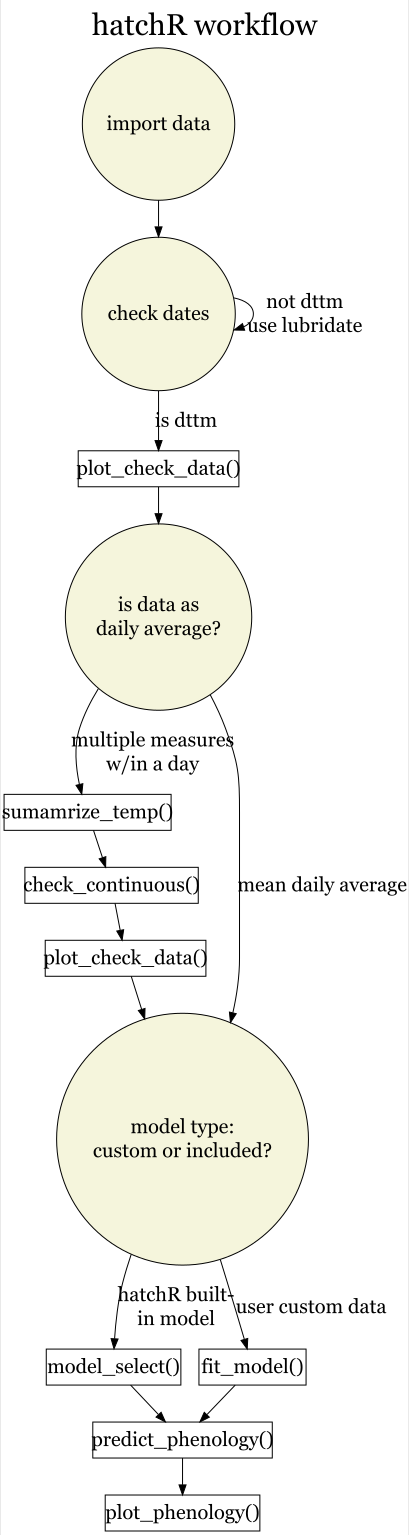
\includegraphics{flowchart.png}

\subsection{Effective value models}\label{effective-value-models}

Effective value models were created by Sparks et al. (2019) to implement
developmental models in wild environments for Sockeye Salmon (\emph{O.
nerka}). The need for change arose because historic models, specifically
those in Beacham \& Murray (1990), only considered the average
incubation temperature during development and, for wild fishes, average
incubation temperature was impossible to estimate because it was unknown
when fish hatched even if adult spawn timing was known. To address this,
Sparks et al. (2019) used the reciprocal of the formulation of model 2
from Beacham \& Murray (1990) and assigned an effective value for every
day of development using the daily average temperature.

The model follows the general format of:

\[
Effective Value_i = 1/exp(log_ea - log_e(Temperature_i - b))
\]

Where \emph{i} is the daily value and a fish hatches or emerges when the
cumulative sum or \[\sum_{i =1}^nEffectiveValue_i = 1\]

The effective value model framework is the basis for the phenological
models in \texttt{hatchR}, both in the included \texttt{model\_table} in
the package, as well as for custom models users can fit with
\texttt{fit\_model()}. Specifically, \texttt{model\_table} has been
extended to include more parameterizations from Beacham \& Murray
(1990), Sparks et al. (2017), and Austin et al. (2019) (who extended
McPhail \& Murray (1979)).

\subsection{Data format}\label{data-format}

\subsection{Checking Data}\label{checking-data}

\texttt{hatchR} is built assuming data will be analyzed as daily average
temperatures. Despite that assumption, raw data (\emph{e.g.}, as
outputted by HOBO loggers) can be used and \texttt{hatchR} includes
functionality to summarize those data into a format that is usable, as
well as provides functions for basic visual and programmatic data checks
to make sure outliers or missing data are at least brought to users'
attention.

summarize\_temp, check\_continuous and plot\_check\_temp

\subsection{Model Selection}\label{model-selection}

talk about using nls for fit\_model

model\_table and fit\_model

fit\_model for three non-salmonid species

\begin{Shaded}
\begin{Highlighting}[]
\NormalTok{smallmouth }\OtherTok{\textless{}{-}} \FunctionTok{matrix}\NormalTok{(}\ConstantTok{NA}\NormalTok{, }\DecValTok{10}\NormalTok{, }\DecValTok{2}\NormalTok{) }\SpecialCharTok{|\textgreater{}} \FunctionTok{tibble}\NormalTok{()}
\FunctionTok{colnames}\NormalTok{(smallmouth) }\OtherTok{\textless{}{-}} \FunctionTok{c}\NormalTok{(}\StringTok{"hours"}\NormalTok{, }\StringTok{"temp\_F"}\NormalTok{)}
\NormalTok{smallmouth}\SpecialCharTok{$}\NormalTok{hours }\OtherTok{\textless{}{-}} \FunctionTok{c}\NormalTok{(}\DecValTok{52}\NormalTok{, }\DecValTok{54}\NormalTok{, }\DecValTok{70}\NormalTok{, }\DecValTok{78}\NormalTok{, }\DecValTok{90}\NormalTok{, }\DecValTok{98}\NormalTok{, }\DecValTok{150}\NormalTok{, }\DecValTok{167}\NormalTok{, }\DecValTok{238}\NormalTok{, }\DecValTok{234}\NormalTok{)}
\NormalTok{smallmouth}\SpecialCharTok{$}\NormalTok{temp\_F }\OtherTok{\textless{}{-}} \FunctionTok{c}\NormalTok{(}\DecValTok{77}\NormalTok{, }\DecValTok{75}\NormalTok{, }\DecValTok{71}\NormalTok{, }\DecValTok{70}\NormalTok{, }\DecValTok{67}\NormalTok{, }\DecValTok{65}\NormalTok{, }\DecValTok{60}\NormalTok{, }\DecValTok{59}\NormalTok{, }\DecValTok{55}\NormalTok{, }\DecValTok{55}\NormalTok{)}

\NormalTok{smallmouth }\OtherTok{\textless{}{-}}\NormalTok{ smallmouth }\SpecialCharTok{|\textgreater{}} 
  \FunctionTok{mutate}\NormalTok{(}\AttributeTok{days =} \FunctionTok{ceiling}\NormalTok{(hours}\SpecialCharTok{/}\DecValTok{24}\NormalTok{),}
         \AttributeTok{temp\_C =}\NormalTok{ (temp\_F }\SpecialCharTok{{-}}\DecValTok{32}\NormalTok{) }\SpecialCharTok{*}\NormalTok{ (}\DecValTok{5}\SpecialCharTok{/}\DecValTok{9}\NormalTok{))}

\FunctionTok{plot}\NormalTok{(smallmouth}\SpecialCharTok{$}\NormalTok{days}\SpecialCharTok{\textasciitilde{}}\NormalTok{smallmouth}\SpecialCharTok{$}\NormalTok{temp\_C)}

\NormalTok{smb\_mod }\OtherTok{\textless{}{-}} \FunctionTok{fit\_model}\NormalTok{(smallmouth,}
                     \AttributeTok{temp =}\NormalTok{ smallmouth}\SpecialCharTok{$}\NormalTok{temp\_C,}
                     \AttributeTok{days =}\NormalTok{ smallmouth}\SpecialCharTok{$}\NormalTok{hours)}
\end{Highlighting}
\end{Shaded}

\subsection{Predicting Phenology and
Output}\label{predicting-phenology-and-output}

Use woody \_example from website

show predict\_phenology output slots

show plot\_phenology

\section{Case Study 1}\label{case-study-1}

A common management scenario where developmental phenology might be
useful would be trying to understand if fish might be free-moving before
some management action. For instance, will have fish have emerged from
redds when a stream section has been opened to grazing or bridge
decommissioning will commence?

In this scenario, we will consider the grazing example and Bull Trout, a
threatened fish in the united states under the Endangered Species Act
(Nolfi, Melbihess, Fisher, \& Ellis, 2024), and the East Fork Salmon
River, a key Bull Trout population in the upper Salmon River watershed.
The fisheries manager there wants to know if fish will likely be out of
the gravel and free-swimming by June 1st. In this system, it is expected
that Bull Trout will be done spawning by the end of September, so we'll
consider the last possible spawn date as September 30th.

\begin{Shaded}
\begin{Highlighting}[]
\DocumentationTok{\#\#\# read in EFS data}

\NormalTok{EFS\_data }\OtherTok{\textless{}{-}}\NormalTok{ crooked\_river}

\DocumentationTok{\#\#\# view bull trout models and select model}

\NormalTok{model\_table }\SpecialCharTok{|\textgreater{}} 
  \FunctionTok{filter}\NormalTok{(species }\SpecialCharTok{==} \StringTok{"bull trout"}\NormalTok{)}
\end{Highlighting}
\end{Shaded}

\begin{verbatim}
## # A tibble: 2 x 5
##   author             species    model dev.type func                       
##   <chr>              <chr>      <chr> <chr>    <chr>                      
## 1 Austin et al. 2017 bull trout MM    hatch    1/exp(5.086 - (x * 0.131)) 
## 2 Austin et al. 2017 bull trout MM    emerge   1/exp(5.590 - (x  * 0.126))
\end{verbatim}

\begin{Shaded}
\begin{Highlighting}[]
\CommentTok{\# we care about when fish are out of gravel, so select emerge mod}
\NormalTok{bt\_emerge\_mod }\OtherTok{\textless{}{-}} \FunctionTok{model\_select}\NormalTok{(}\AttributeTok{author =} \StringTok{"Austin et al. 2017"}\NormalTok{,}
                            \AttributeTok{species =} \StringTok{"bull trout"}\NormalTok{,}
                            \AttributeTok{model =} \StringTok{"MM"}\NormalTok{,}
                            \AttributeTok{dev.type =} \StringTok{"emerge"}\NormalTok{)}

\CommentTok{\# predict emergence time using Sept. 30 as the spawn date }
\NormalTok{bt\_emergence }\OtherTok{\textless{}{-}} \FunctionTok{predict\_phenology}\NormalTok{(}\AttributeTok{data =}\NormalTok{ EFS\_data,}
                                  \AttributeTok{dates =}\NormalTok{ date,}
                                  \AttributeTok{temperature =}\NormalTok{ temp\_c,}
                                  \AttributeTok{spawn.date =} \StringTok{"2011{-}09{-}30"}\NormalTok{, }
                                  \AttributeTok{model =}\NormalTok{ bt\_emerge\_mod)}

\CommentTok{\# fish emerge May 1, before June 1}
\NormalTok{bt\_emergence}\SpecialCharTok{$}\NormalTok{dev.period}\SpecialCharTok{$}\NormalTok{stop}
\end{Highlighting}
\end{Shaded}

\begin{verbatim}
## [1] "2012-05-01 UTC"
\end{verbatim}

In this example we expect the last fish out of the gravel well before
the June 1st date and the manager could allow grazing in this area
without worrying about direct mechanical disturbance to fish developing
in the gravel.

\section{Case Study 2}\label{case-study-2}

\section{Discussion}\label{discussion}

talk about how these models also represent local adaptation and
heritable plasticity

talk about how these models represent point estimates and that emergence
and hatch will take the form of a distribution

\section{Acknowledgements}\label{acknowledgements}

We would like to sincerely thank the editor and reviewers for all of
their helpful feedback which greatly improved both the software and the
manuscript.

The views expressed in this manuscript are those of the authors and do
not necessarily represent the views or policies of USFS or USFWS. Any
mention of trade names, products, or services does not imply an
endorsement by the U.S. government, USFS, or USFWS. USFS and USFWS do
not endorse any commercial products, services or enterprises.

\section*{References}\label{references}
\addcontentsline{toc}{section}{References}

\phantomsection\label{refs}
\begin{CSLReferences}{1}{0}
\bibitem[\citeproctext]{ref-adelfio2019}
Adelfio, L. A., Wondzell, S. M., Mantua, N. J., \& Reeves, G. H. (2019).
Warm winters reduce landscape-scale variability in the duration of egg
incubation for coho salmon (oncorhynchus kisutch) on the copper river
delta, alaska. \emph{Canadian Journal of Fisheries and Aquatic
Sciences}, \emph{76}(8), 1362--1375.
doi:\href{https://doi.org/10.1139/cjfas-2018-0152}{10.1139/cjfas-2018-0152}

\bibitem[\citeproctext]{ref-adelfio2024}
Adelfio, L. A., Wondzell, S. M., Mantua, N. J., \& Reeves, G. H. (2024).
Expanded, compressed, or equal? Interactions between spawning window and
stream thermal regime generate three responses in modeled juvenile
emergence for pacific salmon. \emph{Canadian Journal of Fisheries and
Aquatic Sciences}.
doi:\href{https://doi.org/10.1139/cjfas-2023-0238}{10.1139/cjfas-2023-0238}

\bibitem[\citeproctext]{ref-austin2019}
Austin, C. S., Essington, T. E., \& Quinn, T. P. (2019). Spawning and
emergence phenology of bull trout Salvelinus confluentus under differing
thermal regimes. \emph{Journal of Fish Biology}, \emph{94}(1), 191--195.
doi:\href{https://doi.org/10.1111/jfb.13864}{10.1111/jfb.13864}

\bibitem[\citeproctext]{ref-beacham1990}
Beacham, T. D., \& Murray, C. B. (1990). Temperature, egg size, and
development of embryos and alevins of five species of pacific salmon: A
comparative analysis. \emph{Transactions of the American Fisheries
Society}, \emph{119}(6), 927--945.
doi:\href{https://doi.org/10.1577/1548-8659(1990)119\%3C0927:TESADO\%3E2.3.CO;2}{10.1577/1548-8659(1990)119\textless0927:TESADO\textgreater2.3.CO;2}

\bibitem[\citeproctext]{ref-kaylor2021}
Kaylor, M. J., Justice, C., Armstrong, J. B., Staton, B. A., Burns, L.
A., Sedell, E., \& White, S. M. (2021). Temperature, emergence phenology
and consumption drive seasonal shifts in fish growth and production
across riverscapes. \emph{Journal of Animal Ecology}, \emph{90}(7),
1727--1741.
doi:\href{https://doi.org/10.1111/1365-2656.13491}{10.1111/1365-2656.13491}

\bibitem[\citeproctext]{ref-mcphail1979}
McPhail, J., \& Murray, C. (1979). \emph{The early life-history and
ecology of dolly varden (salvelimus malma) in the upper arrow lakes}.
Nelson, BC, Canada.

\bibitem[\citeproctext]{ref-nolfi2024}
Nolfi, D., Melbihess, T., Fisher, S., \& Ellis, L. (2024). 5-Year
Statuse Review Coterminous United States Population of Bull Trout
(Salvelinus confluentus).

\bibitem[\citeproctext]{ref-sparks2019}
Sparks, M. M., Falke, J. A., Quinn, T. P., Adkison, M. D., Schindler, D.
E., Bartz, K., Young, D., et al. (2019). Influences of spawning timing,
water temperature, and climatic warming on early life history phenology
in western alaska sockeye salmon. \emph{Canadian Journal of Fisheries
and Aquatic Sciences}, \emph{76}(1), 123--135.
doi:\href{https://doi.org/10.1139/cjfas-2017-0468}{10.1139/cjfas-2017-0468}

\bibitem[\citeproctext]{ref-sparks2017}
Sparks, M. M., Westley, P. A. H., Falke, J. A., \& Quinn, T. P. (2017).
Thermal adaptation and phenotypic plasticity in a warming world:
Insights from common garden experiments on Alaskan sockeye salmon.
\emph{Global Change Biology}, \emph{23}(12), 5203--5217.
doi:\href{https://doi.org/10.1111/gcb.13782}{10.1111/gcb.13782}

\end{CSLReferences}

\end{document}
